% Script: AISearchAgentDAG.tex
\documentclass{standalone}

\usepackage{amsmath}
\usepackage{xcolor} % Added for color definitions
\usepackage{tikz}
\usetikzlibrary{
    arrows.meta,
    positioning,
    shapes.geometric
}

\begin{document}

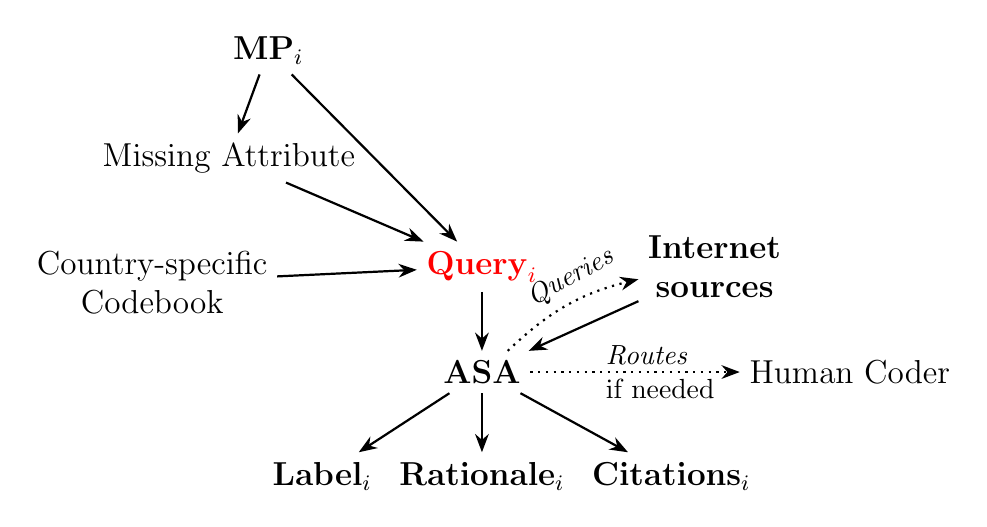
\begin{tikzpicture}[
    ->,
    >=Stealth,
    node distance=0.75cm and 0.66cm,
    node_style/.style={
        align=center,
        font=\large
    },
    edge_style/.style={
        draw=black,
        thick
    }
]

% --- Nodes ---
\node[node_style] (B) {$\mathbf{MP}_i$};
\node[node_style, below=of B,xshift=-0.5cm] (Y) {Missing Attribute};
\node[node_style, below left=of Y,xshift=3cm] (M) {Country-specific\\Codebook};

% Query stays red
\node[node_style, red, below right=of Y] (W) {$\mathbf{Query}_i$};

% Place ASA where Internet used to be (below Query)
\node[node_style, below=of W] (ASA) {$\mathbf{ASA}$};

% Move Internet sources to the right of Query
\node[node_style, right=of W, xshift=0.5cm, align=center] (Internet) {$\mathbf{Internet}$ \\ \textbf{sources}};

% Terminal nodes
\node[node_style, below=of ASA] (WDesc) {$\mathbf{Rationale}_i$};
\node[node_style, below left=of ASA] (WSummary) {$\mathbf{Label}_i$};
\node[node_style, below right=of ASA] (WTrace) {$\mathbf{Citations}_i$};
\node[node_style, right=of ASA,xshift=2cm] (Human) {Human Coder};

% --- Edges ---
\draw[edge_style] (B) -> (Y);
\draw[edge_style] (B) -> (W);
\draw[edge_style] (Y) -> (W);
\draw[edge_style] (M) -> (W);

% Query only has an arrow going into ASA
\draw[edge_style] (W) -> (ASA);

% ASA to Internet (unidirectional; not bidirectional)
\draw[edge_style,dotted] (ASA) to [bend left=15]
    node[above, sloped, xshift=0.2cm,align=center] {{\it Queries}} (Internet);

% ASA outputs
\draw[edge_style] (Internet) -> (ASA);
\draw[edge_style] (ASA) -> (WTrace);
\draw[edge_style] (ASA) -> (WSummary);
\draw[edge_style] (ASA) -> (WDesc);
\draw[edge_style,dotted] (ASA) -- (Human) node[midway, right, align=left,xshift=-0.5cm] {\it Routes \\if needed};

\end{tikzpicture}

\end{document}
